\documentclass{beamer}
\usepackage{beamerthemesplit}
\usepackage{wrapfig}
\usetheme{SPbGU}
\usepackage{pdfpages}
\usepackage{amsmath}
\usepackage{cmap} 
\usepackage[T2A]{fontenc} 
\usepackage[utf8]{inputenc}
\usepackage[english,russian]{babel}
\usepackage{indentfirst}
\usepackage{amsmath}
\usepackage{tikz}
\usepackage{multirow}
\usepackage[noend]{algpseudocode}
\usepackage{algorithm}
\usepackage{algorithmicx}
\usetikzlibrary{shapes,arrows}
\usepackage{fancyvrb}
\newtheorem{rutheorem}{Теорема}
\newtheorem{ruproof}{Доказательство}
\newtheorem{rudefinition}{Определение}
\newtheorem{rulemma}{Лемма}
\beamertemplatenavigationsymbolsempty

\title[]{Доработка алгоритма синтаксического анализа регулярной аппроксимации кода на встроенных языках}
\subtitle[]{YaccConstructor}
% То, что в квадратных скобках, отображается в левом нижнем углу. 
\institute[]{
Лаборатория языковых инструментов JetBrains \\
Санкт-Петербургский государственный университет \\
Математико-механический факультет }

% То, что в квадратных скобках, отображается в левом нижнем углу.
\author[Екатерина Вербицкая]{Екатерина Вербицкая}

\date{10 сентября 2015г.}

\definecolor{orange}{RGB}{179,36,31}

\begin{document}
{
\begin{frame}[fragile]
  \begin{tabular}{p{2.5cm} p{5.5cm} p{2cm}}
   \begin{center}
      
\includegraphics[width=2.5cm]{../../../2014/SECR/slides/JBLogoWhite.png}
    \end{center}
    &
    \begin{center}
      
\includegraphics[width=1cm]{pictures/SPbGU_Logo.png}
    \end{center}
    &
    \begin{center}
      
\includegraphics[width=1cm]{pictures/YC_big.jpg}
    \end{center} 
  \end{tabular}
  \titlepage
\end{frame}
}

\begin{frame}[fragile]
  \transwipe[direction=90]
  \frametitle{YaccConstructor}
  \begin{itemize}
    \item Проект для исследований в области лексического и синтаксического 
анализа
    \item Открытый исходный код
    \begin{itemize}
      \item \url{https://github.com/YaccConstructor/YaccConstructor}
    \end{itemize}
    \item Основной язык разработки --- F\#
  \end{itemize}
\end{frame}
            
\begin{frame}
  \transwipe[direction=90]
  \frametitle{Алгоритм}
  \begin{itemize}
    \item Синтаксический анализ \textbf{всех строк} из регулярного 
\textbf{множества}
    \item Вход --- не одна строка, а множество (возможно бесконечное)
    \item Множество описано конечным автоматом
  \end{itemize}
\end{frame}

\begin{frame}[fragile]
  \transwipe[direction=90]
  \frametitle{Сфера применимости алгоритма}
\begin{tabular}{p{4.5cm} p{8cm}}
Встроенный код
&
\begin{minipage}[t]{5cm}

\begin{Verbatim}[commandchars=\\\{\}]
\textcolor{blue}{string} res = \textcolor{orange}{""};
\textcolor{blue}{for}(i = 0; i < l; i++)
    res = \textcolor{orange}{"()"} + res;
\fbox{\textcolor{blue}{use}(res);}

\end{Verbatim}
\end{minipage}

\\ 
Возможные значения
&
\begin{minipage}[t]{2.5cm}
\begin{Verbatim}[commandchars=\\\{\}]
\{\textcolor{orange}{""}, \textcolor{orange}{"()"},  \textcolor{orange}{"()()"}, ..., \textcolor{orange}{"()"}^l\}
\end{Verbatim}
\end{minipage}

\\
Аппроксимация
&
\begin{minipage}[t]{4cm}
  \begin{Verbatim}[commandchars=\\\{\}]
(\textcolor{orange}{"()"})*
  \end{Verbatim} 
\end{minipage}

\\
Соответствующий КА
&
\begin{minipage}[t]{3cm}                        
\raisebox{-\height}{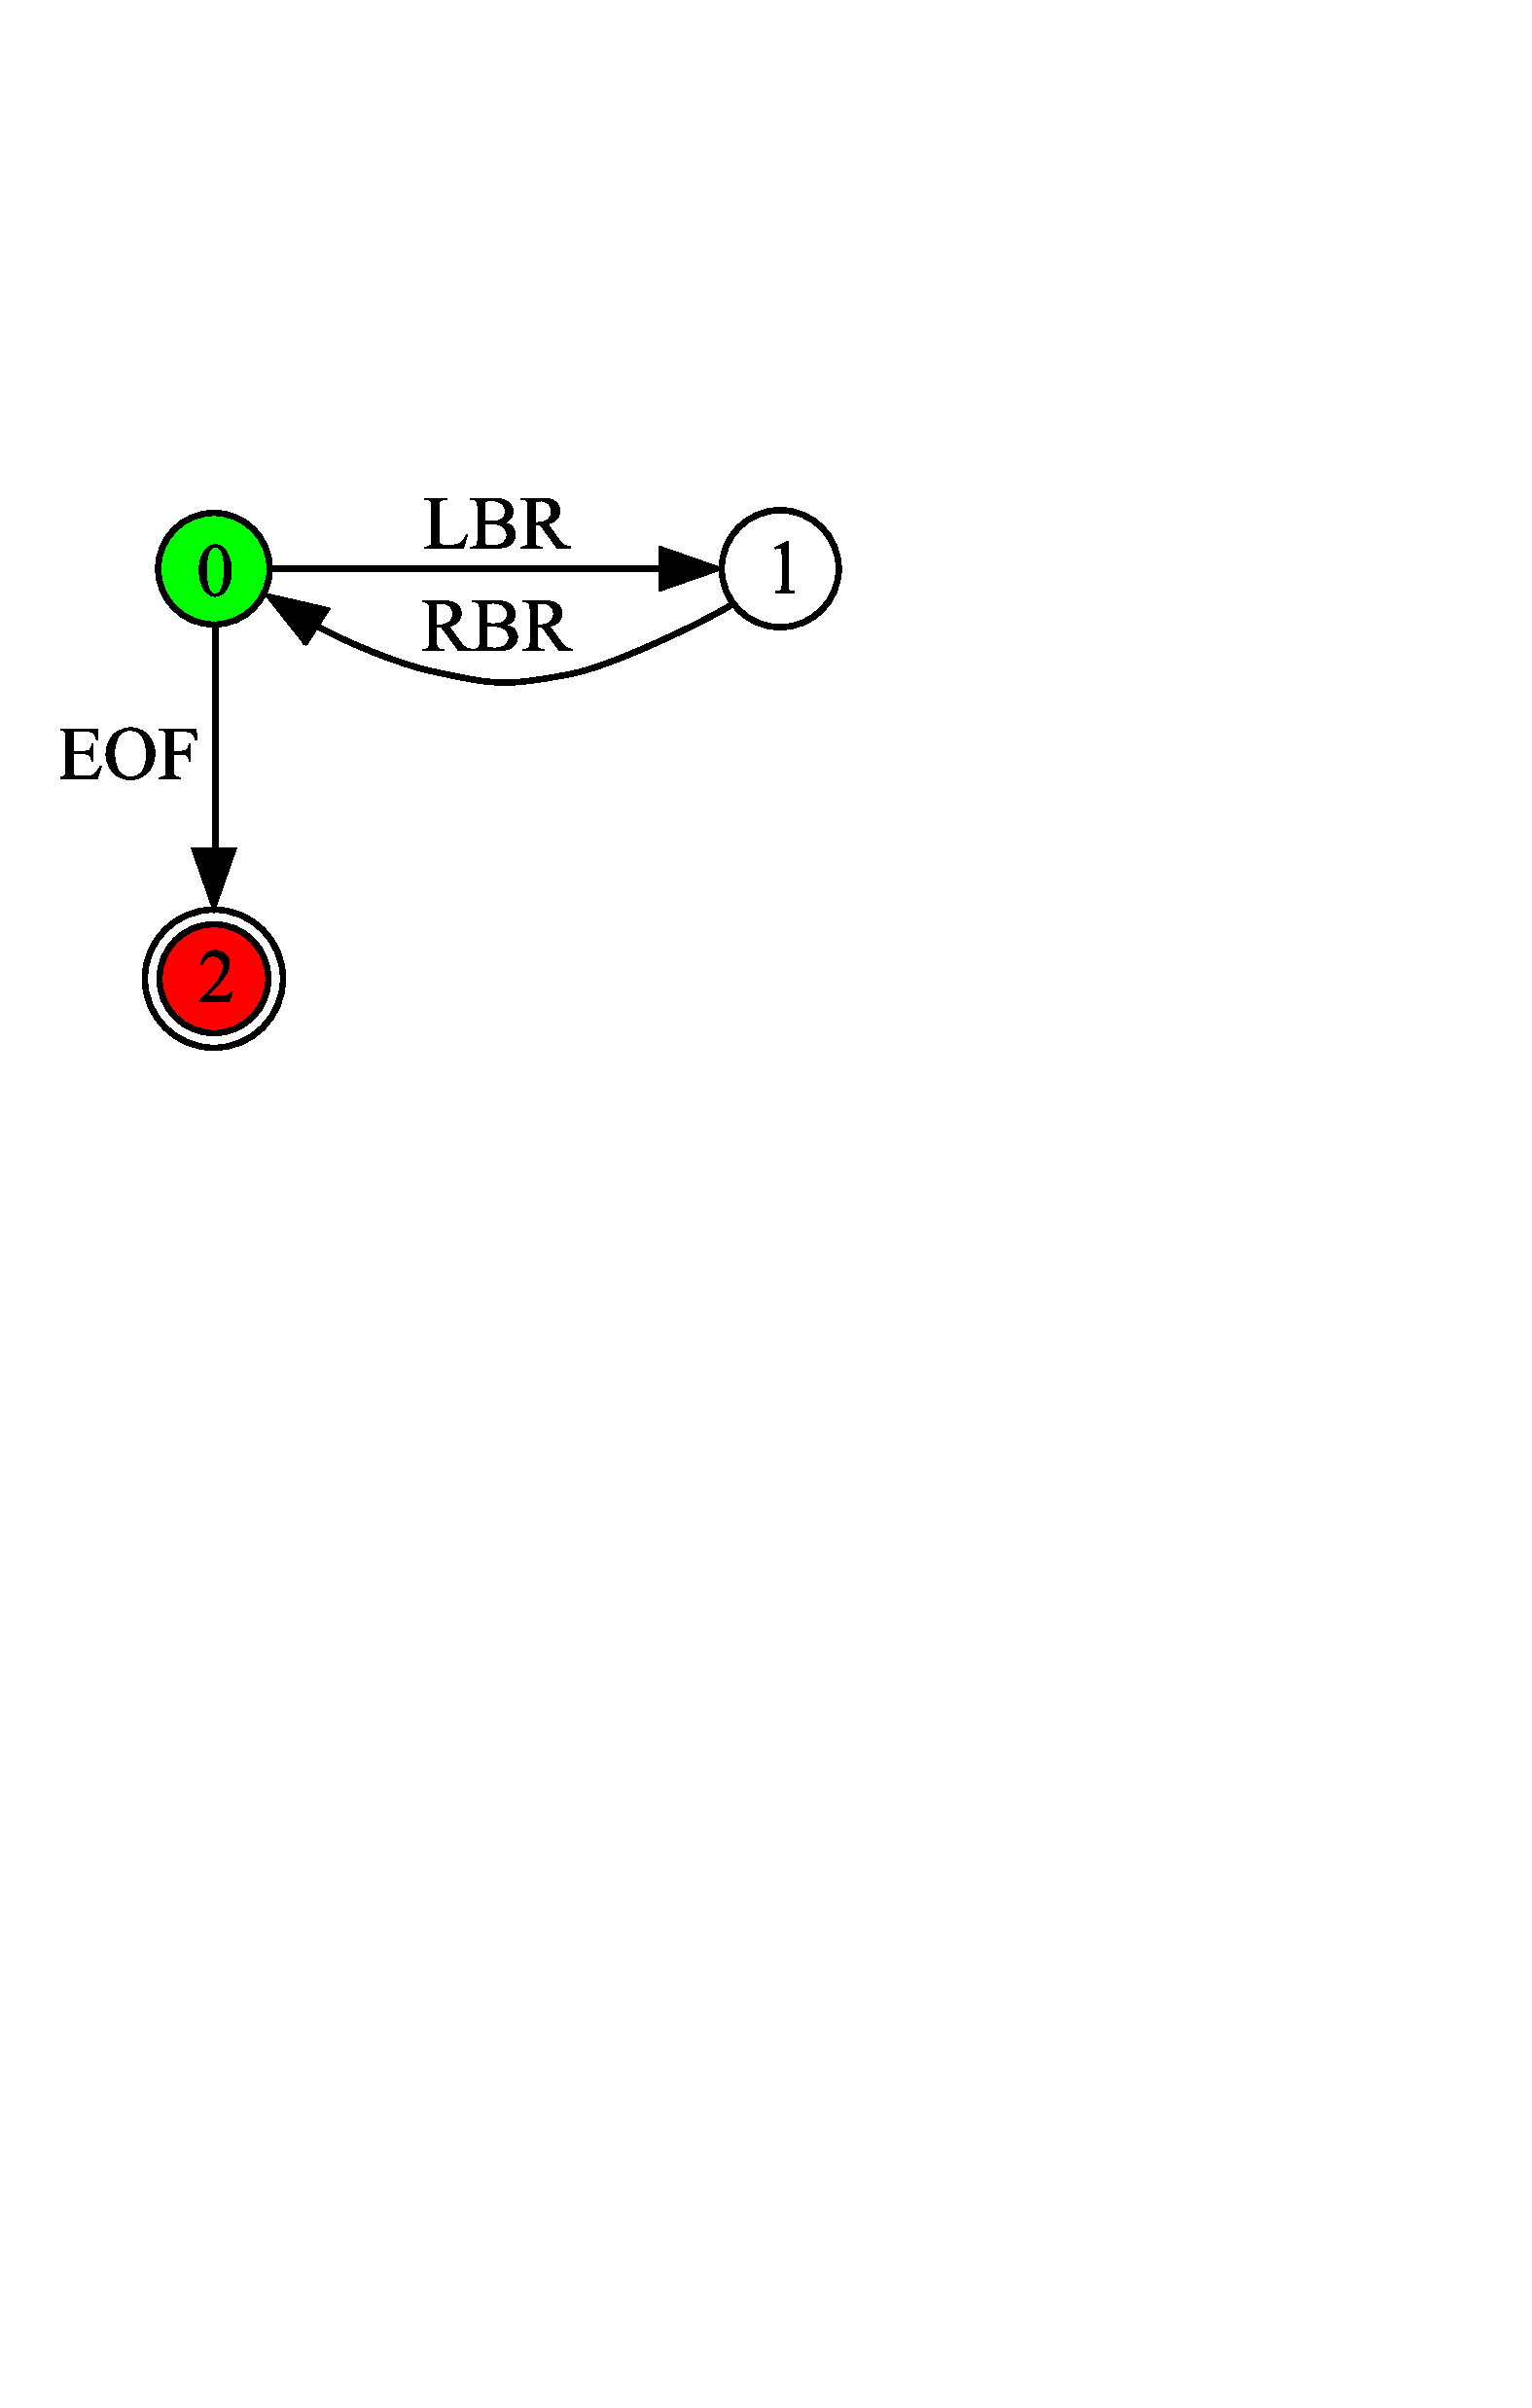
\includegraphics[width=3cm]{../../../2015/PSI/slides/pictures/in31}}
\end{minipage}


\end{tabular}

\end{frame}


\begin{frame}
  \transwipe[direction=90]
  \frametitle{Задача: ослабить ограничения на входной автомат}
  \begin{itemize}
    \item Детерминированный автомат без $\epsilon$-переходов $\Rightarrow$ произвольный 
конечный автомат
  \end{itemize}
  \begin{itemize}
    \item Несложная задача на семестр
  \end{itemize}
\end{frame}

\begin{frame}
  \transwipe[direction=90]
  \frametitle{Задача: диагностика и сообщение об ошибках}
  \begin{itemize}
    \item Предлагается 2 подхода
    \item На диплом: реализовать и сравнить оба подхода
    \item Можно разделить на 2 человек
    \item Результаты можно будет опубликовать
  \end{itemize}
\end{frame}

\begin{frame}
  \transwipe[direction=90]
  \frametitle{Требования к знаниям и навыкам}
  \begin{itemize}
    \item Знакомство с функциональным программированием
    \begin{itemize}
      \item Знание F\# или OCaml является преимуществом
    \end{itemize}
    \item Базовые знания в области синтаксического анализа
  \end{itemize}
\end{frame}


\begin{frame}
\transwipe[direction=90]
\frametitle{Контакты}
\begin{itemize}
  \item Почта: \url{kajigor@gmail.com}
  \item Исходный код YaccConstructor: \url{https://github.com/YaccConstructor/YaccConstructor}
  \item Google+ сообщество: \url{https://goo.gl/DuPWkM}
  \item Больше задач на GitHub: \\ \small{\url{https://github.com/YaccConstructor/YaccConstructor/issues}}
\end{itemize}
\end{frame}
\end{document}
